\chapter{Affective Computing}

\section{Definizione e Concetti}
L'Affective Computing è il campo di studio che si occupa dello sviluppo di sistemi in grado di riconoscere, interpretare, processare e simulare le emozioni umane.

\subsection{Modelli Categorici (Discreti) delle Emozioni}
Prima di passare a modelli continui, la teoria psicologica ha storicamente definito le emozioni tramite categorie discrete universali:
\begin{itemize}
    \item \textbf{Modello di Ekman:} Identifica \textbf{6 emozioni di base} universali trans-culturali: Gioia, Tristezza, Rabbia, Paura, Disgusto e Sorpresa, rintracciabili tramite micro-espressioni facciali.
    \item \textbf{Ruota di Plutchik:} Estende il modello a \textbf{8 emozioni primarie} organizzate in coppie di opposti (Es. Gioia/Tristezza, Fiducia/Disgusto, Paura/Rabbia, Sorpresa/Anticipazione). Le emozioni complesse derivano dalla fusione di queste primarie.
\end{itemize}

\section{Analisi dell'Arousal e della Valenza (Circumplex Model di Russell)}
Per dare una classificazione continua alle emozioni, piuttosto che appoggiarsi a categorie base (e.g. gioia, rabbia, tristezza, paura, disgusto, sorpresa di Ekman), ci si basa storicamente sul modello circonflesso introdotto da Russell nel 1980. Esso mappa le sensazioni umane su uno spazio bidimensionale continuo:
\begin{itemize}
    \item \textbf{Asse Y - Arousal (Attivazione):} Grado dell'energia associata all'emozione (Es. Basso: dormiente / Alto: frenetico, allertato).
    \item \textbf{Asse X - Valence (Valenza):} Disposizione qualitativa o umore (Es. Basso: spiacevole, negativo / Alto: piacevole, positivo).
\end{itemize}

\vspace{0.5cm}
\begin{figure}[h!]
    \centering
    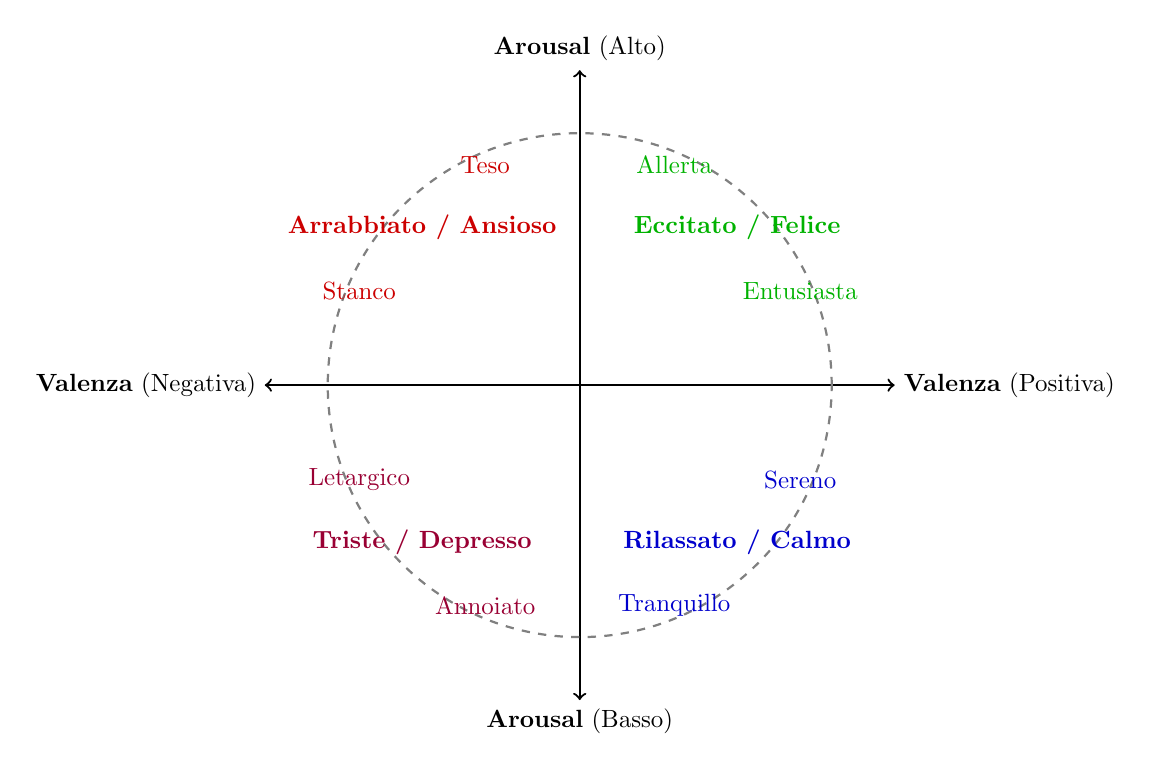
\begin{tikzpicture}[scale=0.8, every node/.style={scale=0.9}]
        % Assi
        \draw[<->, thick] (-5,0) -- (5,0) node[right] {\textbf{Valenza} (Positiva)};
        \draw[<->, thick] (0,-5) -- (0,5) node[above] {\textbf{Arousal} (Alto)};

        \node[left] at (-5,0) {\textbf{Valenza} (Negativa)};
        \node[below] at (0,-5) {\textbf{Arousal} (Basso)};

        % Cerchio base
        \draw[thick, dashed, gray] (0,0) circle (4cm);

        % Quadrante 1 (Alto Arousal, Alta Valenza)
        \node[text=green!70!black, font=\bfseries] at (2.5, 2.5) {Eccitato / Felice};
        \node[text=green!70!black] at (1.5, 3.5) {Allerta};
        \node[text=green!70!black] at (3.5, 1.5) {Entusiasta};

        % Quadrante 2 (Alto Arousal, Bassa Valenza)
        \node[text=red!80!black, font=\bfseries] at (-2.5, 2.5) {Arrabbiato / Ansioso};
        \node[text=red!80!black] at (-1.5, 3.5) {Teso};
        \node[text=red!80!black] at (-3.5, 1.5) {Stanco};

        % Quadrante 3 (Basso Arousal, Bassa Valenza)
        \node[text=purple!80!black, font=\bfseries] at (-2.5, -2.5) {Triste / Depresso};
        \node[text=purple!80!black] at (-3.5, -1.5) {Letargico};
        \node[text=purple!80!black] at (-1.5, -3.5) {Annoiato};

        % Quadrante 4 (Basso Arousal, Alta Valenza)
        \node[text=blue!80!black, font=\bfseries] at (2.5, -2.5) {Rilassato / Calmo};
        \node[text=blue!80!black] at (3.5, -1.5) {Sereno};
        \node[text=blue!80!black] at (1.5, -3.5) {Tranquillo};

    \end{tikzpicture}
    \caption{Il Modello Circonflesso delle Emozioni (Russell, 1980).}
\end{figure}
\vspace{0.5cm}

Ad esempio, alta valenza e alto arousal corrispondono all'eccitazione/felicità (Happy), mentre bassa valenza e alto arousal ricadono sotto stress emotivi come ansia o rabbia (Angry).

\section{Il Dataset DEAP e gli Standard di Riferimento}
Per fornire benchmark validi sulle macchine di classificazione emozionale (spesso affrontate in ambito \textit{Affective BCI}) è stato standardizzato il \textbf{DEAP Dataset} (Database for Emotion Analysis using Physiological Signals).

\subsection{Dettagli dell'Esperimento DEAP}
L'esperimento DEAP è una pietra miliare configurata con estremo rigore:
\begin{itemize}
    \item \textbf{Partecipanti e Stimoli:} 32 partecipanti hanno visionato 40 video musicali della durata di 1 minuto ciascuno, precedentemente selezionati tramite i tag affettivi del sito \textit{Last.fm} per coprire uniformemente i vari quadranti emotivi.
    \item \textbf{Acquisizione dati:} Registrazione multimodale che include EEG (32 canali), segnali periferici associati al sistema nervoso autonomo (GSR, temperatura corporea, frequenza respiratoria, ECG, fotopletismogramma) e per 22 partecipanti anche le espressioni facciali su video.
    \item \textbf{Ground Truth e SAM:} Come si etichettano le emozioni intime in un dataset? Ai candidati veniva chiesto di compilare una scala \textbf{SAM (Self-Assessment Manikin)} per fornire l'autovalutazione di \emph{Arousal, Valenza, Dominanza} e \emph{Liking}. In questo ambito è cruciale la differenza tra \textbf{emozioni espresse} (il soggetto "mostra" un'emozione, magari simulata) ed \textbf{emozioni suscitate} o \emph{felt emotions} (ciò che il soggetto "sente" realmente in risposta allo stimolo musicale), di cui il SAM cattura la \textit{ground truth}.
    \item \textbf{Modality Fusion:} La vera innovazione dell'approccio risiede nella fusione decisionale (\textit{decision/modality fusion}): i modelli di machine learning raggiungono le performance migliori non usando il singolo segnale, ma incrociando i dati cerebrali con quelli del sudore o del battito e del volto.
\end{itemize}

Questa fusione di dati multicanale biologici ha reso accessibile l'allenamento di task algoritmici predittivi sul reale stato emozionale del soggetto al computer, con importanti ricadute in settori quali salute mentale pre-clinica (e.g. detection ansia), User Experience, ed intrattenimento (ad esempio dinamiche di giochi modificate dalle reazioni biologiche misurate del giocatore).

\section{Limiti e Prospettive}
A differenza del tracking del mouse o della frequenza di click usati nei convenzionali tool di software tracking, la biologia non mente: per il soggetto risulta arduo alterarne le micro-reazioni (\textit{lie-detector principle}). Questo porta ad un incredibile margine di veridicità del dato acquisito ad una velocità real-time, ma contemporaneamente il suo grosso limite è la scalabilità: ogni candidato porta variazioni intra-soggetto per cui i modelli non riescono sempre a "generalizzare" un approccio universale ma necessitano della fase di calibrazione \textit{in-situ}.
